%----------------------------------------------------------------
%
%  File    :  prediction_model.tex
%
%  Authors : Thomas Lerchbaumer
% 
%  Created :  19 March 2022
% 
%  Changed :  19 March
% 
%----------------------------------------------------------------

\chapter{Predicting Future Bookings}
The knowledge of potential future bookings provide useful insights when it comes to yield management. Yield management in general describes controlling price and capacity control in a simultaneous ways \cite{yield_m}. Therefore those predictions can be used to support bus operators in their pricing strategy.  This chapter focuses on creating two prediction models utilizing different techniques based on the data that is available. 
Both models are implemented using python and the following libraries. 
\begin{itemize}
\item  \verb|matplotlib|\footnote{https://matplotlib.org/} - used for plotting
\item \verb|pandas|\footnote{https://pandas.pydata.org/} - used for data manipulation 
\item \verb|tesnorflow|\footnote{https://www.tensorflow.org/} - provides ML models
\item \verb|keras|\footnote{https://keras.io/} - Neural Network library
\end{itemize}

As there are various models available a literature review was conducted to figure out which models fit the purpose of time series forecasting. It turns out that the most promising NN that can be utilized for time series prediction are either Convolutional Neural Networks (CNN) or Recurrent Neural Networks (RNN) especially Long Short-Term Memory (LSTM)\cite{nn_1}\cite{nn_2}\cite{lstm_1}\cite{lstm_2}.

\section{The Models}
Both models CNN and RNN/LSTM can be used for time series forecasting. To create accurate prediction models a basic knowledge about models functionality is required. Therefore this section explains the components of each NN as well as the approaches those models follow. 

\subsection{LSTM}
LSTM is an RNN and was invented by \cite{lstm_inventor} in 1997. Until today this NN is widley used for time series forecasting and provides reliable results for short as well as long term predictions \cite{rnn_moharm}. LSTM have so called memory cells which are responsible to store the state of data. Whenever information arrives at a memory cell its outcome is defined by refreshing the cell state with the newly arrived information. LSTM utilizes gates to control a cells state by either including or excluding information \cite{lstm_stock}. Those gates are called: 
\begin{itemize}
\item input gate - data selection and storage for upcoming state
\item forget gate - data selection and storage which will not be used for the upcoming state
\item output gate - sets information within the state that is send to the output
\end{itemize}
Those gates are created by combining sigmoid functions. The results of this gates are values ranging from zero to one. A result of zero indicates the cell to not pass any infomration whereas values close to one indicates the cell to pass all information. 
The LSTM Module or Repeating module consits of four NN layers which interact together as shown in Figure \ref{fig:lstm_rep_model}.


\begin{figure}[H]
	\centering
		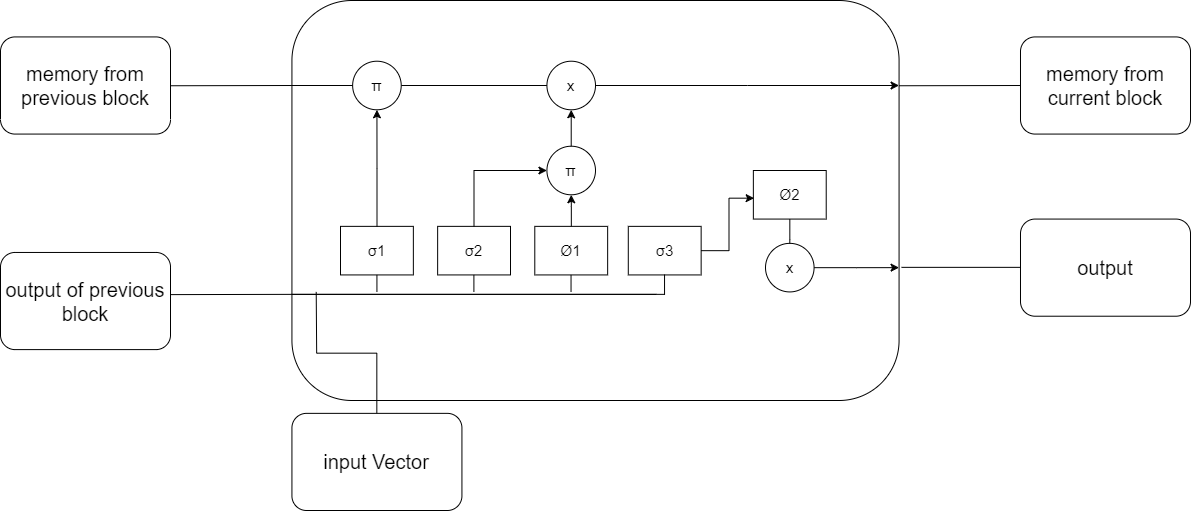
\includegraphics[width=14cm]{images/lstm_module}
	\caption{Repeating LSTM Module - [source:\cite{lstm_module}]}
	\label{fig:lstm_rep_model}
\end{figure}




\subsection{CNN}


\section{Implementation}


\section{Reliability Comparison - LSTM, CNN}

\section{Model accuracy}
Having a look at the model performance accuracy (comparing predictions of the model with already available data) , explain potential twerks that have been applied to the model itself to achieve a higher level of accuracy.

